\section{Introduction}

\begin{frame}{Java is Vulnerable}
	\begin{columns}
		\column{0.55\textwidth}
			As one of the most widely used languages on the planet, a lot of security critical code is written in Java.\newline
		
			Due to its prevalence on the desktop, mobile and (formerly) the web, vulnerabilities in Java can have massive impact.\newline
			
			13 `critical' vulnerabilities were discovered in the JDK last year \cite{nvd:jdk2016cvss9}.
		\column{0.45\textwidth}
		\begin{figure}
			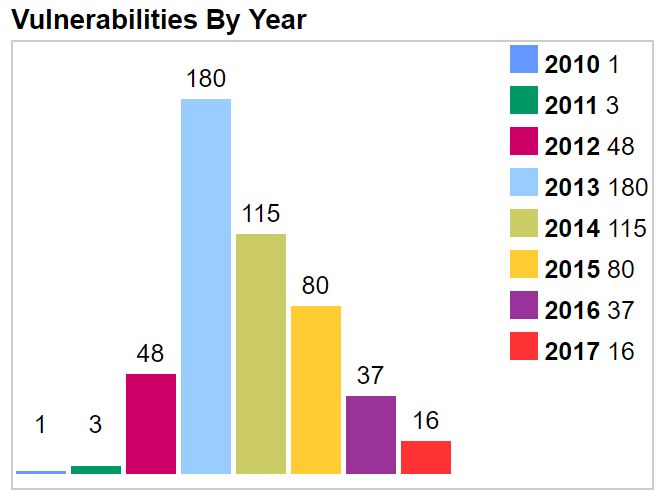
\includegraphics[scale=0.25]{content/images/cvedetails_vulnsperyear.png}
			\caption{Total CVEs by year \cite{cvedetails:jdk2016}}
		\end{figure}
	\end{columns}	
\end{frame}

\begin{frame}{Writing Secure Java Code}
	Developers of security conscious Java applications must ensure the Confidentiality, Integrity and Availability of data. They can do this by:
	
	\begin{itemize}
		\item Following the Oracle Secure Coding Guidelines
		\item Running their application with a \texttt{SecurityManager} installed
		\item Following the Principle of Least Privilege
	\end{itemize}
	
	What they can't usually do is \textit{prove it}.
\end{frame}

\begin{frame}{Thesis Topic}
	One avenue for providing \textit{provable} Confidentiality and Integrity to programs is applying the theory of \textit{Information Flow}.
	
	This leads to the key question this thesis aims to address:
	
	\begin{block}{Key Thesis Question}
		Can Information Flow be used to provide practical improvements to the Confidentiality and Integrity of Java programs?
	\end{block}
\end{frame}

\begin{frame}{Thesis Overview}
	\begin{block}{Key Thesis Question}
		Can Information Flow be used to provide practical improvements to the Confidentiality and Integrity of Java programs?
	\end{block}

	To answer this question, 
\end{frame}